% MIT License
%
% Copyright (c) 2021 Geoffrey H. Garrett
%
% Permission is hereby granted, free of charge, to any person obtaining a copy
% of this software and associated documentation files (the "Software"), to deal
% in the Software without restriction, including without limitation the rights
% to use, copy, modify, merge, publish, distribute, sublicense, and/or sell
% copies of the Software, and to permit persons to whom the Software is
% furnished to do so, subject to the following conditions:
%
% The above copyright notice and this permission notice shall be included in all
% copies or substantial portions of the Software.
%
% THE SOFTWARE IS PROVIDED "AS IS", WITHOUT WARRANTY OF ANY KIND, EXPRESS OR
% IMPLIED, INCLUDING BUT NOT LIMITED TO THE WARRANTIES OF MERCHANTABILITY,
% FITNESS FOR A PARTICULAR PURPOSE AND NONINFRINGEMENT. IN NO EVENT SHALL THE
% AUTHORS OR COPYRIGHT HOLDERS BE LIABLE FOR ANY CLAIM, DAMAGES OR OTHER
% LIABILITY, WHETHER IN AN ACTION OF CONTRACT, TORT OR OTHERWISE, ARISING FROM,
% OUT OF OR IN CONNECTION WITH THE SOFTWARE OR THE USE OR OTHER DEALINGS IN THE
% SOFTWARE.

%%%%%%%%%%%%%%%%%%%%%%%%%%%%%%%%%%%%%%%%%%%%%%%%%%%%%%%%%%%%%%%%%%%%%%%%%%%%%%%
% ACKNOWLEDGEMENTS
%%%%%%%%%%%%%%%%%%%%%%%%%%%%%%%%%%%%%%%%%%%%%%%%%%%%%%%%%%%%%%%%%%%%%%%%%%%%%%%
% Adapted from:
% https://www.researchgate.net/figure/The-agent-environment-interaction-in-reinforcement-learning_fig1_328494763

%%%%%%%%%%%%%%%%%%%%%%%%%%%%%%%%%%%%%%%%%%%%%%%%%%%%%%%%%%%%%%%%%%%%%%%%%%%%%%%
% DEPENDENCIES
%%%%%%%%%%%%%%%%%%%%%%%%%%%%%%%%%%%%%%%%%%%%%%%%%%%%%%%%%%%%%%%%%%%%%%%%%%%%%%%
%\usepackage{tikz}
%\usetikzlibrary{decorations.pathreplacing}    % for TikZ braces
%\usetikzlibrary{positioning}                  % for TikZ relative positioning

%%%%%%%%%%%%%%%%%%%%%%%%%%%%%%%%%%%%%%%%%%%%%%%%%%%%%%%%%%%%%%%%%%%%%%%%%%%%%%%
% USER STYLING
%%%%%%%%%%%%%%%%%%%%%%%%%%%%%%%%%%%%%%%%%%%%%%%%%%%%%%%%%%%%%%%%%%%%%%%%%%%%%%%

% TikZ node design.
\tikzset{basic/.style={draw,text width=1em,text badly centered}}
\tikzset{input/.style={basic, fill=green!25, circle}}
\tikzset{output/.style={basic, fill=blue!25, circle}}
\tikzset{weight/.style={basic,circle}}
\tikzset{hidden/.style={basic,circle}}
\tikzset{function/.style={basic,circle}}

%%%%%%%%%%%%%%%%%%%%%%%%%%%%%%%%%%%%%%%%%%%%%%%%%%%%%%%%%%%%%%%%%%%%%%%%%%%%%%%
% TIKZ PICTURE
%%%%%%%%%%%%%%%%%%%%%%%%%%%%%%%%%%%%%%%%%%%%%%%%%%%%%%%%%%%%%%%%%%%%%%%%%%%%%%%
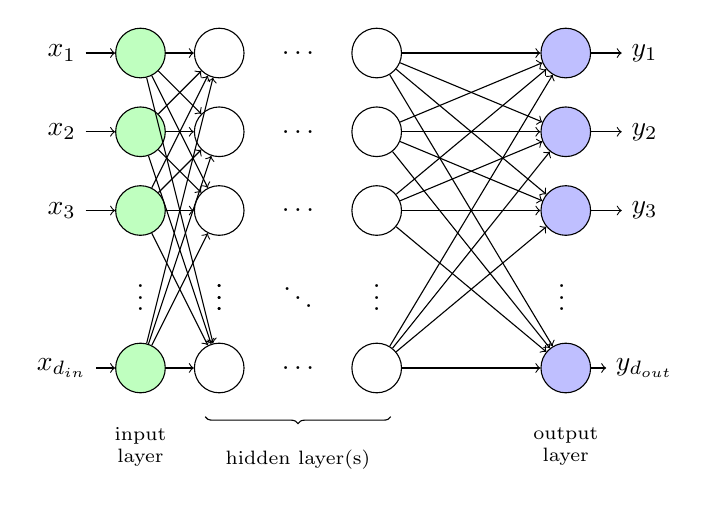
\begin{tikzpicture}
    \usetikzlibrary{decorations.pathreplacing}    % for TikZ braces
    \usetikzlibrary{positioning}                  % for TikZ relative positioning

    % input
    \foreach \n/\p in {0/1,1/2,2/3,3/4,4/5} {
        \ifnum \n=3
            % dots layer
            \node[] at (0, -\n) (X_\n) {$\vdots$};
            \node[] at (\hiddenx, -\n) (H1_\n) {$\vdots$};
            \node[right of=H1_\n] (M-\n) {$\ddots$};
            \node[below of=H1_2] (H2_\n) {$\vdots$};
            \node[below of=H2_2] (H2_\n) {$\vdots$};
            \node[right=5.7em of H2_\n] (Y_\n) {$\vdots$};
        \else
        \ifnum \n=4
            % n layer
            \node[input] at (0, -\n) (X_\n) {};
            \node[left of=X_\n] (I_\n) {$x_{d_{{in}}}$};
            \path[draw,->] (I_\n) -- (X_\n);
            \node[hidden] at (\hiddenx, -\n) (H1_\n) {}; %{$h_{n, 1}$};
            \node[right of= H1_\n] (M-\n) {$\ldots$};
            \node[hidden, right of= M-\n] (H2_\n) {}; % {$h_{n, m}$};
            \node[output, right= 5em of H2_\n] (Y_\n) {}; % {$h_{n, m}$};
            \node[right of=Y_\n] (O_\n) {$y_{d_{out}}$};
            \path[draw,->] (Y_\n) -- (O_\n);
        \else
            \node[input] at (0, -{\n}) (X_\n) {};
            \node[left of=X_\n] (I_\n) {$x_{\p}$};
            \path[draw,->] (I_\n) -- (X_\n);
            \node[hidden] at (\hiddenx, -\n) (H1_\n) {};%{$h_{\n, 1}$};
            \node[right of=H1_\n] (M-\n) {$\ldots$};
            \node[hidden, right of=M-\n] (H2_\n) {};% {$h_{\n, m}$};
            \node[output, right= 5em of H2_\n] (Y_\n) {}; % {$h_{n, m}$};
            \node[right of=Y_\n] (O_\n) {$y_\p$};
            \path[draw,->] (Y_\n) -- (O_\n);
        \fi
        \fi
    }

    % input layer connected to first hidden layer
    \foreach \j in {0,1,2,4} {
        \foreach \n in {0,1,2,4} {
            \path[draw,->] (X_\n) -- (H1_\j);
        }
    }

    % second hidden layer connected to output layer
    \foreach \j in {0,1,2,4} {
        \foreach \n in {0,1,2,4} {
            \path[draw,->] (H2_\n) -- (Y_\j);
        }
    }

    % labels
    \node[below of=X_4,font=\scriptsize, align=center] {input\\layer};
    \node[below of=Y_4,font=\scriptsize, align=center] {output\\layer};

    % brace for hidden layers
    \node[below=1em of M-4] (hidden-brace) {};
    \node[right=3em of hidden-brace] (hidden-brace-right) {};
    \node[left=3em of hidden-brace] (hidden-brace-left) {};
    \draw [decorate,decoration = {brace}] (hidden-brace-right) --  (hidden-brace-left);
    \node[below=0.5em of hidden-brace,font=\scriptsize] (hlayer) {hidden layer(s)};

\end{tikzpicture}

